\chapter{Introduction}  %Title of the First Chapter

The observation that human traits are heritable is evident, often visible by eye. 
Every one of us has been told that they have their mother’s eyes, their father’s height, their grandfather’s nose, etc. 
Similarly, many diseases “run in the family”: for example diabetes, or some types of breast cancer, are recurrent from generation to generation. 
In fact, for some conditions, family history can be one of the most reliable diagnostic tools. 
Describing the mechanisms by which we acquire traits, and the extent to which traits are heritable is at the core of the science we now call genetics, and is a question that has occupied scientists for years.

%********************************** %First Section  **************************************
\section{From peas to GWAS}  %Section - 1.1 

%********************************** % 1.1.1  **************************************
\subsection{Principles of (Mendelian) Inheritance} %Section - 1.1.1 

In On the Origin of Species \cite{darwin1859origin}, Charles Darwin proposed the theory of evolution, which is based on the assumption that natural variation between individuals provides differential reproductive advantages, and that this variation can be inherited from one generation to the next. 
This theory nicely explains the adaptation of a species to its environment and the consequent development of new species, yet the mechanisms by which such variation occurs and the modes of inheritance were not described. 
In the words of Darwin himself in On the Origin of Species: “Our ignorance of the laws of variation is profound” and “The laws governing inheritance are quite unknown” \cite{darwin1859origin}.\\

Around the same time, specifically in 1853, the man who is now universally considered to be the father of genetics began conducting experiments to tackle this problem exactly. 
He was actually not a scientist but a friar, by the name of Gregor Mendel, and he was going to perform the now infamous experiments on inheritance in peas. 
At St. Thomas’ abbey, in Brno, Moravia (then part of the Austro-Hungarian empire), Mendel meticulously studied seven different traits of the plants (plant height, pod shape and color, seed shape and color, and flower position and color), each of which segregated on one of the plant's seven chromosomes. 
For example, seeds were either yellow or green, wrinkled or round. For seven years, Mendel followed generations and generations of pea plants and noted that some traits occurred far more often than others. 
For example, when crossing a plant with round seeds and one with wrinkled seeds, the offspring ($F_1$) always had round seeds: Mendel called the round seed trait the “dominant” trait. However, the wrinkled seed trait that had seemingly vanished in the first filial generation would appear again, in the second generation ($F_2$) in a 1 wrinkle seed plant to 3 round seed plants ratio. Somehow, this “recessive” trait was being passed on, remaining hidden when overpowered by the dominant trait, but not forgotten. 
In 1866, Mendel published his experiments and results in "Versuche über Pflanzenhybriden" (Experiments in Plant Hybridization, \cite{mendel1996experiments}). 
In it, he proposes what will be called the Mendelian Laws of Inheritance: i) the Law of Independent Segregation (every individual contains two factors for each trait one of which is passed on to its offspring at random), ii) the Law of Independent Assortment (traits are inherited independently of each other) and iii) the Law of Dominance (recessive alleles will be masked by dominant alleles and the trait corresponding to the dominant allele will be observed) \cite{mendel1996experiments}. 
The publication received almost no attention, but his Laws of Inheritance described therein will build the foundations of modern genetics.\\

Mendel and Darwin never met, and remained unaware of each other’s theories until their deaths. Mendel’s research remained completely unknown for decades, until at the turn of the century in 1900 four botanists (Austrian Erich von Tschermak, Dutchman Hugo de Vries, German Carl Correns and American William Jasper Spillman) independently re-discovered his work and validated his findings, officially beginning the modern age of genetics.\\ 

Around the same time, the British geneticist William Bateson set out to make Mendel’s work accessible to scientists that were not proficient in Mendel’s native language German.
He translated Mendel’s original papers on the Laws of Inheritance into English and published them, allowing Mendel’s work to become known in the greater scientific world (ref), more than 40 years after their original publication.\\ 

An important step towards reconciling Darwin’s theory of evolution with Mendel’s laws of inheritance was made in 1902, when Theodor Boveri showed, in sea urchin, that different chromosomes contained different hereditary material and that organisms required a full set of chromosomes to function. 
In 1903, Walter Sutton published a paper proposing how these principles, together with the random segregation of paternal and maternal chromosomes during gamete formation (which he studied in grasshoppers) could form the molecular basis for Mendel’s Laws of Inheritance (Sutton, 1903). 
Importantly, he also noted how the number of traits was much larger than the number of chromosomes, which meant that some traits had to be located on the same chromosome and be transmitted together.

\subsection{Genetic Linkage and the birth of modern genetics} %Section - 1.1.2 

In 1908, American geneticist Thomas Hunt Morgan set out to confirm (or disprove) Mendel’s theories using a model organism that generates new offspring much quicker than pea plants. 
It was \textit{Drosophila melanogaster}, the fruit fly. 
In his famous “fly room” at Columbia University, thousands of experiments were performed on flies. 
Flies with known phenotypes (such as red eyes) were put in jars to mate, and the traits of the progeny were recorded. 
Through the key observations that some traits appeared to be sex-linked and that some other traits were co-occurring more often than expected by chance, Morgan theorised that “markers” responsible for particular traits were positioned on chromosomes, like beads on a string. 
These markers, or genes (Box 1), when close together on a chromosome were more likely to be passed on to the next generation. 
Morgan had described the concept of genetic linkage and essentially hypothesized the phenomenon of crossing over (exchange of paternal and maternal chromosomal material during meiosis; Morgan, 1911). 
In 1913 his brilliant student, Alfred Sturtevant gathered all the data collected until then and developed the first genetic map, showing the position of the fruit fly’s known markers (or genes) relative to each other in terms of recombination frequency (Sturtevant, 1913). 
Sturtevant will go on to call the unit of genetic linkage a “centimorgan”, in honour of his mentor.\\

The Mendelian-chromosome theory, first proposed by Boveri and Sutton (Sutton, 1903) and then elaborated and expanded by Morgan and his students (Morgan et al., 1915) described chromosomes as the (paired) units of heredity that Mendel had described in his laws, and was widely accepted by scientists by the 1930s. 
In 1933, Morgan received the Nobel Prize in Physiology or Medicine “for his discoveries concerning the role played by the chromosome in heredity”.\\

However, the mechanisms of heredity and the physical molecule responsible for it was still unknown. 
The concept of “gene” existed, but it was an abstract entity. 
Most people in fact believed that proteins were the carriers of genetic material. 
In 1943, Erwin  Schrödinger, an Austrian-Irish physicist better known for his contributions to quantum mechanics, published “What is Life?” where he introduced the idea that genetic material may be stored as some sort of a “code”, a concept borrowed from Information Theory. 
He had provided a theoretical physical description of the mechanism of “storage” of genetic material.\\ 

Still, as most scientists at the time, Schrödinger bet on proteins as the responsible molecule. 
The other candidate, \gls{dna} had been referred to as the “stupid molecule”, a molecule with a chemical structure far too simple to be able to explain the complexity of life. 
In fact, \gls{dna} consists of only four building blocks, often referred to by their initials: adenine (A), thymine (T), cytosine (C) and guanine (G).\\

Proteins remained the most likely responsible for carrying genetic information until 1944, when Oswald Avery and colleagues at the Rockefeller Institute in New York demonstrated experimentally that it had to be \gls{dna}. 
Avery, along with his co-workers Colin MacLeod and Maclyn McCarthy performed an experiment in \textit{Streptococcus pneumoniae}, where he removed various organic compounds from the bacteria, and observed whether it could still transform. 
Only upon treating the bacteria with an enzyme that removed \gls{dna}, the bacteria stopped transforming.

%%%% Box on genetic terms & origin

\begin{Comment}
\hspace{-2.5mm}\textbf{Box 1: Genetic terms}\label{box1}
% \small
\begin{itemize}
    \item Phenotype
    \item Gene
    \item Allele

\end{itemize}


\end{Comment}


\subsection{The double helix} %Section - 1.1.3

The question of the physical structure of the \gls{dna} remained unsolved until in 1953 a team of remarkable scientists proposed one structure. 
Key members of this team were Francis Crick, James Watson, Rosalind Franklin, Maurice Wilkins and Erwin Chargaff. 
Jim Watson had had a fascination for the structure of \gls{dna}, and had been studying it for years, starting in his native Chicago, then during his PhD in Indiana (under the supervision of Italian future Nobel Prize laureate Salvador Luria), to then end up at the Lucy Cavendish laboratory, then directed by Australian-born British X-ray crystallographer Sir Lawrence Bragg, in Cambridge, United Kingdom. 
There, he met Francis Crick, 12 years his senior, a brilliant British physicist turned biologist. 
Crick had taught himself the mathematical theory of X-ray crystallography and had worked on determining the most stable helical conformation of amino acid chains in proteins, the alpha helix, only to be beaten to its solution by American chemist Linus Pauling. 
Watson and Crick set out to obtain a model for the structure of \gls{dna}, building on Crick’s experience and rigor, and Watson’s intuition. 
Friend and collaborator of the pair was Maurice Wilkins, New Zealand-born British physicist at King’s College London, who had extensively studied X-ray diffraction patterns. 
His colleague, Rosalind Franklin had perfected the technique to produce X-ray crystallography images of the \gls{dna} and instructed her assistant, Raymond Gosling, to take the most precise of them to date, the now famous “Photo 51”. 
To Watson and Crick’s eyes, Photo 51 (which Wilkins had shared without Franklin knowing), looked without a doubt like the shadow that a helix would leave. The last piece of the puzzle came from a discovery that Austro-Hungarian Erwin Chargaff made, at Columbia University. He observed that globally the amounts of As and Ts in \gls{dna} were roughly the same, as were the amounts of Cs and Gs. 
This provided the idea that bases would be paired up and facing inwards in the double helix, As with Ts, Cs with Gs, ensuring that the covalent bonds would be always of the same length, keeping the helix stable. 
In 1953, Watson and Crick published “Molecular structure of nucleic acids” (Watson and Crick, 1953). 
Their work showed how the four nucleotide bases (A, T, C, G) formed “two helical chains each coiled round the same axis” (Watson and Crick, 1953) spelling out what Crick called “the secret of life.” 
For this discovery, Crick, Watson and Wilkins won the 1962 Nobel Prize in Physiology or Medicine “for their discoveries concerning the molecular structure of nucleic acids and its significance for information transfer in living material”. 
Rosalind Franklin, who had played a critical role in the discovery had died four years prior of ovarian cancer, and her contribution went largely unrecognized at the time.


\subsection{Biometrics} %Section - 1.1.4
While Mendel was studying the inheritance of traits in peas, whilst Boveri studied sea urchins, Morgan fruit flies, Avery bacteria, and long before Crick, Watson and Franklin proposed a structure for \gls{dna} (working on squid), ever since Darwin’s theories, others were trying to quantify inheritance in the context of human traits.\\ 

One investigator among them was Francis Galton, a half-cousin of Darwin’s, who was interested in mathematically describing and analysing Darwin’s evolutionary concepts. 
He was particularly fascinated by the question of how evolution applied to humanity and how its effects could be used to improve the human race. 
To this end, Galton applied himself to the study of biometrics, trying to measure and estimate the heritability of human traits such as height and mental capabilities.\\ 

Linked to these efforts, and on a less honourable note, Galton was also the founder of eugenics, a theory for which genetics should be used as a tool to force evolution’s hand by encouraging mating of individuals considered to have especially desirable qualities and on the other hand by eliminating or preventing reproduction of individuals considered faulted. Eugenics theories are linked to one of the most horrifying pages of human history, motivating forced sterilizations of the “unfit” in the United States in the 1920s and 1930s and of course having being used as justification for the racial policies of Nazi Germany.\\ 

Nevertheless, some of the concepts and methods Galton developed during these studies are still fundamental to genetics today (Galton, 1909). 
These include the concepts of correlation, regression toward the mean and the regression line, which Galton used to compare the heights of children to those of their parents. Galton’s protégé was the mathematician Karl Pearson, who worked together with Galton to make several more important contributions to statistics. Among others, he introduced the concepts of the p-value and the chi squared test (Pearson, 1900) and proposed principal component analysis (PCA, Pearson, 1901).

\subsection{Towards quantitative genetics} %Section - 1.1.5

By cross-breeding Drosophila lines and performing genetic mapping, Morgan and his students had conducted the first genotype-phenotype studies. 
Similar to Mendel and Bateson the phenotypes they observed were predominantly categorical, such as the colour and shape of seeds in pea plants or the red or white-eyed phenotype in \textit{Drosophila melanogaster}. 
In contrast, biometricians like Galton and Pearson had mostly looked at continuous traits in humans, such as height, and believed that those could not be explained by Mendelian genetics.
This controversy has been referred to as the ‘Biometric-Mendelian debate’.\\ 

This debate was resolved by British statistician Ronald A. Fisher, who in a seminal 1918 paper showed that, if many genes affect a trait, then the random sampling of alleles at each gene produces a continuous, normally distributed phenotype in the population (Fisher, 1918). 
As the number of genes grows very large, the contribution of each gene becomes correspondingly smaller, leading in the limit to Fisher’s famous ‘‘infinitesimal model’’ (Barton et al., 2016).\\

In addition to showing that biometrics and Mendelianism are not contradictory but complementary, Fisher made several contributions to the field, outlining statistical ideas and tools still used today. 
An undergraduate student at the University of Cambridge, Fisher [1912] published his first paper "On a absolute criterion for fitting frequency curves" where he outlined the fundamental ideas of maximum likelihood estimation (MLE). 
He later extended on this work and by 1922, he had established the properties of the maximum likelihood estimator such as consistency and minimum variability [Fisher, 1922b] that is still used today [Hald, 1999]. 
He demonstrated the utility of maximum likelihood estimation in genetics by solving a number of equations to elucidate a genetic map of eight \textit{Drosophila melanogaster} genes based on their crossing-over frequencies [Fisher, 1922d].\\ 

In the same year and years to follow, he published a series of papers where he derived the distribution and significance testing of regression coefficients, correlation ratios and multiple regression coefficients [Fisher, 1922c; Fisher, 1928], an exact test for two-by-two contingency tables with small expectations (Fisher’s exact test) [Fisher, 1922a], partial correlation coefficients [Fisher, 1924b] and the variance ratio, later named after Fisher as the F statistic [Fisher, 1924a]. 

Additionally, in his 1918 work, Fisher introduced the concepts of variance (as “the square root of the mean squared error”) and analysis of variance (ANOVA). 
He employed these concepts during his appointment at Rothamsted Experimental Station where he analysed data from crop experiments that had been produced by the agricultural research institute over many decades.
This work resulted in his series of publications entitled Studies in Crop Variation (see for example Fisher, 1921; Fisher and Mackenzie, 1923). 

In 1930, Fisher published the book "The Genetical Theory of Natural Selection" where he reconciled Darwin’s evolutionary theory of natural selection and Mendel’s inheritance laws. 
He gave the first, comprehensive quantitative theory of sexual selection, evolution of recombination rates, polymorphism and many more concepts found in today’s field of population genetics [Fisher, 1930]. 
Thus, together with J.B.S. Haldane and Sewall Wright, Fisher essentially founded the field of population genetics in the 1930s.\\

A few decades later, building on Fisher’s work, Charles Henderson derived the solution of the mixed model equation (Henderson, 1950). 
Nowadays linear mixed models constitute the standard tool for many genetic analyses and are the basic building block of this thesis.

\subsection{Linkage analysis}

\subsection{Technological advancements}

\subsubsection{\gls{dna} sequencing}
The independent development of two different \gls{dna} sequencing techniques by two groups, one Frederick Sanger and the other Walter Gilbert together with Allan Maxwell, were a further big leap in understanding the biological basis of genetic variation. 
Sanger’s method of \gls{dna} sequencing with chain-terminating inhibitors eventually became the standard for \gls{dna} sequencing and subsequent innovations lead to the development of automatic sequencing machines which allowed for sequencing lengths of about one kilobase. 
For sequencing longer stretches of \gls{dna}, a novel strategy named shotgun sequencing was developed. 
In shotgun sequencing, the long \gls{dna} of interest is randomly broken up into shorter \gls{dna} fragments which are cloned and sequenced separately. 
The occurrence of overlapping \gls{dna} fragments given by the random nature of creating the short fragments allows for the in silico reconstruction of longer \gls{dna} fragments.
In 1995, the first genome of a living organism –the bacteria \textit{H. influenzae}– was sequenced and assembled by shotgun sequencing. 
The genomes of other model organisms were to follow in subsequent years (yeast [Goffeau et al., 1996], C. elegans [C. elegans Sequencing Consortium, 1998], D. melanogaster [Adams et al., 2000]) until the first draft of the human genome was published in 2001 [International Human Genome Sequencing Consortium, 2001].
The sequence of the human genome, the development of faster, massively-parallel next-generation sequencing techniques (reviewed in [Shendure et Ji, 2008; Heather et Chain, 2016]) and \gls{dna} microarrays that allow for the genotyping of hundreds of thousands of genetic markers simultaneously [Wang et al., 1998], started a new era of human genetic and genomic research.


\subsubsection{Genotype mapping}

\subsection{The Human Genome Project}

A driving force behind the growth and success of genetic association studies has been technological evolution; breakthroughs in \gls{dna} sequencing and genotyping have pushed human disease research forward, inducing a shift in the field each time technological
advances are introduced to the market. 
The first major breakthrough to dramatically change the landscape of genetics was the Human Genome Project (HGP), which United States President Clinton referred to as "an epic-making triumph of science and reason" (Clinton, 2000) at the announcement of its completion.\\

After the White House announcement in 2000 and a first publication in 2001, the 
project was truly completed on April 25th, 2003, on the 50th anniversary years of the Watson and Crick paper describing the helical structure of \gls{dna}.
the HGP provided the first map of the ~3 billion bases in the human genome (Lander et al., 2001; Schmutz et al., 2004; Hattori, 2005). 
The HGP was a massive international undertaking and a truly collaborative effort; sequencing and analysis took place across twenty centers in six different countries (USA, UK, France, Germany, Japan, China) and took 13 years to complete, costing approximately \$2.7 billion (National Human Genome Research Institute, 2003b).\\ 

Additional breakthroughs in sequencing technologies have expanded and refined the reference genome, which now captures more than 92\% of the genome and provides a landscape of its 20,000 genes (Lander, 2011a).\\

With a complete map of the human genome in place, it was now easy to identify genetic
variants, those bases discovered in an individual that did not match the (reference) base
annotated in the map of the human genome. More common (minor allele frequency >5\%) variants were called single nucleotide polymorphisms (SNPs). 
Previous studies had estimated that approximately 0.1\% (1 base per 1,000) of an individual's genome was a polymorphism (Li and Sadler, 1991; Wang, 1998; Cargill et al., 1999). 
Most of these polymorphisms were scattered across the genome and no one had yet broadly described what these variants were, where in the genome they resided, and what (if any) phenotypic effect they conferred.\\

The International HapMap Project, launched in October of 2002, was the first effort of its
kind to systematically catalogue such variation (The International HapMap Consortium et al., 2003). 
By genotyping individuals of European, African and East Asian descent, HapMap assembled the first phase (2005) of a publicly available database of common variants (>5\% frequency) in global samples (The International HapMap Consortium, 2005). 
The HapMap expanded rapidly. 
By Phase II (2007), the database contained 2.1 million SNPs from four different populations (Frazer et al., 2007); Phase III (2010) added genotyping from seven additional populations, for a total of >3 million SNPs in 11 populations (Altshuler et al., 2010). 
With the map of the genome complete and cataloguing efforts moving apace, researchers could now begin to search for modest effect genetic variants associated to human disease across the full length of the genome.

\subsection{Genotype-phenotype studies}
\subsubsection{Genetic linkage analyses}

Huntington's disease (chromosome 4)

Cystic fibrosis (chromosome 7)

\subsubsection{Genome-wide association studies}

The data generated by the International HapMap Project combined with development of appropriate chip-based microarray technology, enabling simultaneous genotyping of more than one million SNPs, led to the first wave of genome-wide association studies (GWAS).

Briefly, GWAS are a hypothesis free approach to test for significant association between the genotype frequency of common genetic variants (one by one across the entire genome) and a trait of interest \cite{mccarthy2008genome}. 

The first successful GWAS conducted in 2005 for age-related macular degeneration (AMD) using 96 cases and 50 healthy controls, tested for associations at ~100,000 SNPs.

In 2007, the Wellcome Trust Case-Control Consortium (WTCCC) published a study where they performed GWAS on seven different common diseases, using a common set of 3,000 healthy controls and 2,000 cases for each of bipolar disorder (BD), coronary artery disease (CAD), Crohn's disease (CD), hypertension (HT), rheumatoid arthritis (RA), type I and II diabetes (T1D, T2D), \cite{wellcome2007genome}.\\ 

Whilst these early GWAS were based on the directly genotyped tag SNPs, from 2008 onwards, utilisation of methods to fill in missing genotype data became increasingly common practice, referred to as imputation (ref). 

Imputation is a statistical technique to infer genotypes. 
The general idea is to compare genotyped samples to a reference panel of individuals of similar ancestry to identify short haplotype stretches that are shared between the genotyped and reference samples (Fig. 1.3b). This then allows missing genotypes to be filled in.
Initially, data from the HapMap Project was used as a reference panel, with for example the CEU panel used to impute samples of European ancestry. 
Imputation is now also used to explore association effects of rare variants (see Section 1.2.1 for further details of imputation of rare variants, including examples of current reference panels used).

Initially, GWAS focused on complex phenotypes with binary outcomes, using a case control design. 
For each SNP and binary trait, the association was therefore often evaluated using a Cochran–Armitage (trend) test
$\chi^2$ test or a Fisher's exact test comparing the numbers of cases and controls when stratified by their allelels at the locus of interest.

Quantitative traits have since become increasingly popular to use as phenotypes. 
% This is partly due to the fact that the onset of many diseases is time dependent, meaning that some individuals selected as controls may later become cases and hence the control group actually contains a mixture of cases and controls, resulting in some loss of power. 
% In addition, some binary traits are defined by thresholding a continuous variable, with the threshold somewhat arbitrary such that an individual with a value marginally greater than the cutoff is said to be `diseased' whilst an individual just below the threshold is defined as `healthy'.
% Examples include defining obesity based on a BMI threshold and diabetes based on fasting glucose levels. 
% This thresholding approach results in loss of information regarding phenotypic similarity and as a result, using the binary outcome is likely to be less powered than using the underlying quantitative trait. 
% Moreover, quantitative traits are often closer to the underlying biology, providing greater insight into the mechanisms underpinning trait or disease development and the results from using continuous traits may be more directly interpretable, in that it is possible to quantify the average difference in trait outcome per risk allele carried.

Furthermore, linear regressions and their derivations have become more popular methods to assess association, due to their flexibility to include covariates (McCarthy, 2008).
I describe these models in detail in the next Chapter (\textbf{Chapter 2}). 

As of 2020 when I am writing this thesis, over 70,000 associations have been identified for over 1,000 different traits and diseases, according to the GWAS Catalog (ref).

Linkage disequilibrium (LD, The nonrandom allocation of alleles at nearby variants to individual chromosomes as a result of recent mutation, genetic drift or selection, manifest as correlations between genotypes at closely linked markers.)

Hardy-Weinberg equilibrium (HWE,A theoretical description of the relationship between genotype and allele frequencies that is based on expectation in a stable population undergoing random mating in the absence of selection, new mutations and gene flow: in the context of genetic studies, departures from equilibrium can be used to highlight genotyping errors.)

\cite{mccarthy2008genome}

GWAS results are often visualised using Manhattan plots, with the negative log P value plotted on the y-axis against the corresponding genomic position ordered by chromosome and position on the x-axis. 
Peaks on these plots represent loci (multiple variants in LD) that display evidence of association with the analysed phenotype. 
Variants are deemed to be significantly associated with a trait if they exceed an appropriately chosen P value threshold. Due to LD structure, if a peak arises from a single variant, this is usually indicative of a false positive finding.

\subsubsection{From case-control to cohort studies}

UK Biobank ~ 500,000 individuals

\subsubsection{Challenges in GWAS}

Rare diseases: often rare variants too (MAF<0.05)
Pleiotropy: same variant affects multiple traits

non-additive interactions:
Epistasis: combined effect of separate variants interacting to have an effect on trait
GxE:interaction between a variant and an environment


\subsection{Genotype-Environment interactions}

Explicitly, whilst a variant with a significant genetic effect is determined by a mean phenotypic difference between groups of individuals with different allele dosages and a significant environment effect is determined by a mean phenotypic shift that is constant across different allele dosages (Fig. 1.6b), a significant statistical interaction effect is defined when there is a significant difference in the genetic effect between two groups of individuals with different environmental exposures.

% \begin{figure}[h]
% \centering
% 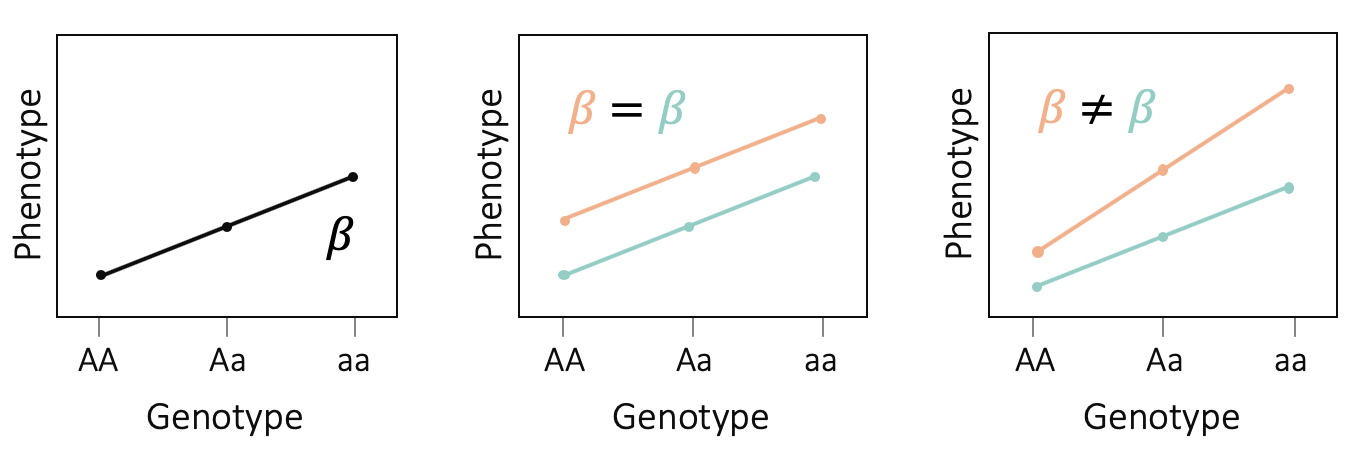
\includegraphics[width=15cm]{Chapter1/Fig/GxE.png}
% \caption{\textbf{Illustration of GxE effect}.\\
% a) Genetic effects only. b) Environments have effects on phenotype but do not change the genetic effect. c) Interaction effect between genotype and environment (GxE).}
% \end{figure}

\newpage

%********************************** %Second Section  **************************************
\section{Gene expression and eQTL mapping}  %Section - 1.2 

\subsection{\gls{dna} and the central dogma}
The resolution of the \gls{dna} structure and all discoveries that lead to it brought forward an understanding of other biological concepts such as protein synthesis and enabled Francis Crick to postulate the central dogma of biology: information is transmitted from nucleic acids (\gls{dna} and RNA) to proteins, but information cannot be transmitted from a protein to \gls{dna} [Crick, 1958]. 
The deciphering of the genetic code through Nirenberg and others followed a few years later [Nirenberg \& Matthaei, 1961; Crick \& al., 1961; Matthaei \& al., 1962].\\

Today, we know that \gls{dna} gets transcribed into RNA aided by the \gls{dna} polymerase molecule, and RNA gets translated to amino-acids making up proteins in the ribosome, with the help of transfer RNA (tRNA).

\subsection{Gene regulation}

In the process of gene expression, the genetic information stored in the \gls{dna} is used to produce molecular products. 
The information on the composition of these products is contained in restricted portions of the genome known as genes. 
In the first step of gene-expression (transcription), genes are transcribed into ribonucleic acid (RNA) molecules. 

Although RNA molecules can be the final product of gene expression, many RNA molecules are translated into proteins in a process known as translation. 
Proteins are long chains of smaller molecules called amino acids. 
Only approximately 1.5\% of the human genome codes for proteins (Lander et al., 2001) while a large fraction of the remaining portion is likely to play a role in the regulation of gene expression (ENCODE Project Consortium, 2004). 

The impact of genetic variation on phenotypes is the consequence of perturbations to this complex molecular machinery.
An easily interpretable mechanism through which genetic variants may affect phenotype is the direct alteration of the structure of the coded protein and thus of its functionality. 
For example, sickle cell anaemia is caused by a SNP in the \textit{HBB} gene, which causes a substitution of an amino acid in the sequence of the coded protein (Laird and Lange, 2010). 
Alternatively, genetic variation may affect the regulation of gene expression. 
One way this can occur is through the disruption of a specific sequence that affects the binding of proteins regulating the expression of a gene, for example a transcription factor (TF). 
Another possibility is the alteration of the structure of the \gls{dna}, thereby affecting the functionality of regulatory elements and ultimately gene expression (ENCODE Project Consortium, 2004; Kundaje et al., 2015). 

\subsection{Estimation of gene expression levels}

In this thesis, we focus on gene expression, i.e., the transcriptome, as a molecular phenotype.
In general, the transcriptome describes the complete set of transcripts in a tissue or cellular sample, and their respective quantity. 
As a precursor of protein expression, mRNA can serve as a proxy of gene expression levels. 
Multiple approaches have been developed to measure cellular mRNA levels, including hybridization- and sequencing-based approaches. 
In the case of hybridization-based methodology, reverse transcription (RT) is used to generate a complementary \gls{dna} (c\gls{dna}) template of the mRNA. 
When this c\gls{dna} template is being amplified with labelled hybridization probes via quantitative polymerase chain reaction (qPCR), fluorescence is emitted according to the oligonucleotides that are being incorporated. 
Based on the fluorescence signal, the genetic sequence of the original mRNA strand can be reconstructed. 
Alternatively, a hybridization microarray contains pre-defined probes for transcripts of every known gene of one or several species. Transcripts that are not known a priori can be detected with tag-based methods such as SAGE (Serial Analysis of Gene Expression); SAGE uses small tags that cover only fragments of a transcript as probes, and can therefore, opposed to hybridization microarray chips, also discover transcripts whose full sequence is unknown. 
However, a large proportion of the tags used by SAGE does not map to unique regions of a reference genome due to their short length, and can therefore not be used for transcript quantification. 
Further, tag-based approaches do not ensure the analysis of the entire transcriptome, and can generally not discover alternative splicing events (Wang et al., 2009).
RNA sequencing (RNA-Seq) based on next-generation sequencing (NGS) of the c\gls{dna} allows for genome-wide quantification of the transcriptome. After obtaining one (single-read RNA-Seq) or two paired (paired-end RNA-Seq) sequence reads per c\gls{dna} fragment, the sequencing reads are either aligned to a reference genome or are assembled de novo. 
From the number of RNASeq reads that map to a particular gene an estimation of gene expression can be deduced. 
In this thesis, we use FPKM (fragments per kilo base per million reads mapped) for gene expression estimations. 
FPKM quantify the number of reads that are assigned to a given gene, normalised by gene length and the total sequencing depth (Wang et al., 2009).
Opposed to the hybridization- and tag-based methods, NGS allows for identifying completely new genes, previously unknown genetic variants in the genes, variation in alternative splicing, or post-transcriptional modifications. In addition, RNA-Seq can quantify the vast array of non-coding RNA molecules (Section 1.1.1). Altogether, sequencing-based assessments of the transcriptome deliver more detailed insights into gene expression variability than hybridization- or tag-based approaches.
In this thesis, we quantify gene expression by RNA-Seq measurements of mRNA levels.

The human genome project revealed that human \gls{dna}
consists of surprisingly few exons (1.1\% of the genome), whereas introns cover 24\% of the genome (Venter et al., 2001; Lander et al., 2001). 
The number of genes was also found to be smaller than expected, with around 30,000 being identified in 2001, and 19,000 genes being the latest estimate at the time that this thesis is written (Ezkurdia et al., 2014). 


\subsection{Expression quantitative trait loci}

The decrease in cost of high-throughput profiling of gene expression has made it possible to measure gene expression levels in large numbers of individuals, thereby enabling the mapping of quantitative trait loci for gene expression (eQTL mapping, Schadt et al., 2003).

As genetic effects on molecular traits may depend on factors such as tissue, environment and cell type, it is necessary to measure expression and other molecular traits in disparate cellular contexts. For this reason, the Genotype-Tissue Expression Project (GTEx Consortium, 2015) has been collecting and analysing gene expression profiles for more than 50 tissue types from over 900 donors.

The latest version of GTEx (v8, ref) assesses eQTL in 53 tissues

In addition, eQTL have been described in iPSC (dicussed later in Section 4)
% add box on overview of tissues with available eQTL

\newpage

%********************************** %Third Section  **************************************
\section{Single cell RNA-seq}  %Section - 1.3 

Next generation sequencing approaches have been applied to individual cells to quantify
variation in \gls{dna} sequence, mRNA expression, epigenetic marks and protein abundance
at single cell resolution.

In this thesis, we focus on gene expression only, and therefore on single cell RNA sequencing (scRNA-seq).

\subsection{Evolution of scRNA-seq technologies}

\subsubsection{Plate-based technologies}

SmartSeq2

\subsubsection{Droplet-based technologies}

DropSeq, 10X Genomics

%\subsection{Analysis of scRNA-seq data}

\subsection{Computational modelling of scRNA-seq}
\subsubsection{Normalization}

\subsubsection{Batch effects}

\subsubsection{Visualization techniques}

scRNA-seq data visualization techniques used in this thesis: 

\begin{itemize}
    \item principal component analysis (PCA)
    \item t-distributed stochastic neighbour embedding (tSNE)-2008 \cite{maaten2008visualizing}
    \item uniform manifold approximation and projection (UMAP)-2018 \cite{mcinnes2018umap}
\end{itemize}

\subsection{General applications of scRNA-seq in biology}

Studies of single-cell transcriptomes allow us to directly investigate properties of individual cells, i.e. mRNA abundance. 
Thus gene regulation is analyzed at the single cell level and, unlike traditional bulk RNA- sequencing, cell-to-cell heterogeneity can be considered.

By measuring gene expression in development, differentiation, or other responses, we can start to understand cellular phenotypes as well as the regulatory processes that determine these phenotypes. 
In many experiments cells are sampled at many time points and gene expression is assessed.

\subsubsection{Atlases}

Human Cell Atlas (HCA)
\subsubsection{Cancer}
\subsubsection{Immunology}
\subsubsection{Development}

\newpage

%********************************** %Fourth Section  **************************************
\section{Human induced pluripotent stem cells}  %Section - 1.4 

\subsection{Early development}

Development

Embryonic stem cells

Organoids

%****** Box on model organisms ******

%\newpage

\begin{Comment}
\hspace{-2.5mm}\textbf{Box 2: Model organisms}\label{box2}\\
% \small

Model organisms are non-human species used to study biological phenomena:

\begin{itemize}
    \item Bacteria (\textit{Escherichia coli}, or \textit{E. coli})
    \item Budding Yeast (\textit{Saccharomyces cerevisiae} or \textit{S. cerevisiae})
    \item Thale cress (\textit{Arabidopsis Thaliana})
    \item Fruit fly (\textit{Drosophila melanogaster})
    \item Nematode worm (\textit{Caenorhabditis elegans} or \textit{C. elegans})
    \item Western clawed frog (\textit{Xenopus tropicalis})
    \item Zebrafish (\textit{Danio rerio})
    \item Mouse (\textit{Mus musculus})

\end{itemize}


\end{Comment}

%**************

\subsection{Stem Cell systems}

(applications for regenerative medicine and disease therapeutics)

\begin{itemize}
    \item ESCs (embryonic stem cells)
    \item TSPSCs (tissue-specific progenitor stem cells)
    \item MSCs (mesenchymal stem cells)
    \item UCSCs (umbilical cord stem cells)
    \item BMSCs (bone marrow stem cells)
    \item iPSCs (induced pluripotent stem cells)
\end{itemize}

list from \cite{mahla2016stem}


add timeline from (Current status of pluripotent stem cells: moving the first therapies to the clinic,  figure 2)

\cite{kimbrel2015current}

\subsubsection{iPSCs}

First developed in mice, it won XX the Nobel prize

Inducing factors:
\textit{OCT4}

%**************

\subsection{iPSC consortia}

\subsubsection{HipSci}
The Human Induced Pluripotent Stem Cell Initiative (HipSci) is the largest of such consortia, and we will use data from HipSci throughout this thesis.

\subsubsection{other iPSC consortia and large studies}

iPScore, Banovich et al

\newpage

\section{Thesis outline}

The overall aim of this thesis is to provide suitable methods to perform eQTL mapping at single cell resolution and to explore the effects of common genetic variants on single cell expression across a range of human iPSC-derived cell types using data from the HipSci project.\\

Specifically, in Chapter 2, I give an overview of current LMMs for genetic analyses, covering their use for association and interaction testing, focusing on their application in eQTL mapping.\\

In Chapter 3, I introduce the two main datasets used in this thesis. \\

In Chapter 4, I present different approaches to mean-level eQTL mapping using scRNA-seq data, and apply them on the data from the two studies described in Chapter 3. \\

In Chapter 5, I present two additional types of QTL analyses we can perform taking advantage of the single cell resolution: interaction QTL and variance QTL. \\

In Chapter 6, we present a novel method to test for multivariate interaction eQTL. \\

Finally, in Chapter 7 I conclude and discuss future directions.